\documentclass{beamer}

\title{\Huge Matrix Project}
\subtitle{\huge EE-1390}

\author{SUNIL VARMA \and EE17BTECH11026 \\  CVS KUSAL REDDY \and EE17BTECH11012}



\usetheme{Singapore}

\begin{document}
\begin{frame}
  \titlepage
\end{frame}
\begin{frame}{\LARGE Geometrical Question}
	
	{\Large The point diametrically opposite to the point $P(1,0)$ on the circle $x^{2}+y^{2}+2x+4y-3=0$ is }
	

\end{frame}

\begin{frame}{\LARGE Matrix Transformation}
	\begin{itemize}
	
	\item {Given circle in matrix form: \\
\begin{centering}
\[\textbf{x} \textbf{x}^T+
\textbf{x}
\begin{bmatrix}
2 \\
4
\end{bmatrix}
=
3
\] \\
  \end{centering}  
                  }
	\end{itemize}
 \end{frame}



\begin{frame}{\LARGE Solution in terms of Matrix}
\begin{itemize}

\item {General equation of circle in matrix form:
\[\textbf{x} \textbf{x}^T 
-
2 \textbf{x} \textbf{c}^{T}
=
r^{2}
-
\textbf{c} \textbf{c}^{T}
\]
} \\

\item {Here,

on comparing with our equation 

-2\textbf{c}^{T} =\begin{bmatrix}
2\\
4

\end{bmatrix}}\\

\item{
Centre of circle \textbf{c} =
\begin{bmatrix}
-1 & -2

\end{bmatrix}
}

\item{r^{2}-\textbf{c} \textbf{c}^{T}
=3}\\

\item{r^{2}-5=3}\\

\item{Radius of circle
r = 2^{3/2} }\\
\end{itemize} \\

\end{frame}

\begin{frame}{Solution contd...}
\begin{itemize}
	\item {Given $P(1,0)$ is the point on the circle } \\
	    
	\item {Let $Q(a,b)$ be the diametrically opposite point to P}  \\ 
	\item{As $Q(a,b)$ lies on circle and diametrically opposite to $P(1,0)$}\\
	
	\item {So  ,} \\
	\item {C is the mid point of  $P(1,0)$ and $Q(a,b)$ }\\
	
\end{itemize}
\end{frame}

\begin{frame}{Solution contd...}
\begin{itemize}

\item{C =\dfrac{P+Q}{2}}\\
\item{Q = 2C-P}
\item{Q = 2$\begin{bmatrix}
-1 & -2\\
\end{bmatrix}$
-
$\begin{bmatrix}
1 & 0\\
\end{bmatrix}$}\\
\item{Q=\begin{bmatrix}
-3 & -4\\
\end{bmatrix}}\\
\item{Therefore ,}\\
\item {Q=\begin{bmatrix}
-3 & -4\\
\end{bmatrix} \hspace{2mm} is\hspace{2mm}  the \hspace{2mm} diametrically\hspace{2mm}  opposite \hspace{2mm} point \hspace{2mm} to\hspace{2mm}  $P(1,0)$ }\\

\end{itemize}
\end{frame}
\begin{frame}{\LARGE Figure}
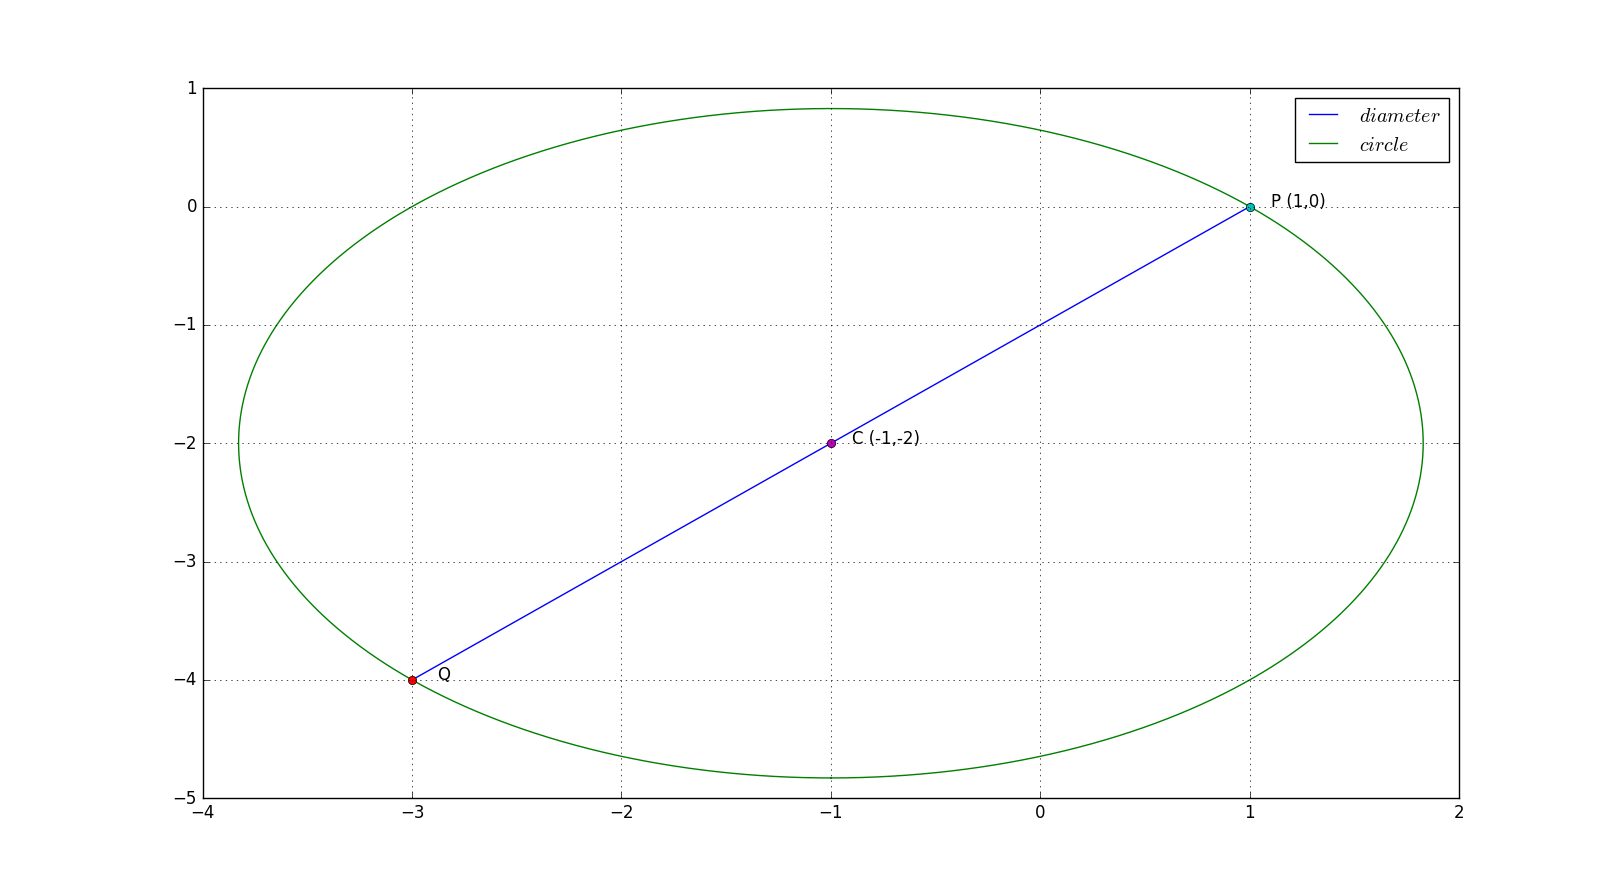
\includegraphics[scale=0.25]{figure_1}
\end{frame}


\end{document}